
    \chapter*{Grids and Numerical Derivatives}
    \addcontentsline{toc}{chapter}{Grids and Numerical Derivatives}
    
    \section*{Introduction to Python}
    \addcontentsline{toc}{section}{Introduction to Python}
  
    In this course we will use Python to study numerical techniques for solving some partial differential equations that arise in Physics. 
    Don\rq t be scared of this new language. 
    Most of the ideas, and some of the syntax, that you learned for Matlab will transfer directly to Python. 
    We\rq ll work through some brief tutorials about Python at the beginning of eachlab, focusing on the particular ideas that you\rq ll need tocomplete 		    that lab. 
    Pretty soon you will be Python wizards. 
    
    
     \begin{problem} \label{P1.1}
      Work through Chapter 1 of Introduction to Python. There you will learn the basics of how to write a Python program, howtodeclare anduseentities called NumPyarrays, and also learn some basic plotting techniques. 
      With that Python knowledge underourbelts, let\rq s move on to begin our study of partial differential equations.
    \end{problem}

    \section*{Spatial grids}
    \addcontentsline{toc}{section}{Spatial grids}
    
    When we solved ordinary differential equations in Physics 330 we were usually moving something forward in time, so you may have the impression that differential equations always \lq flow\rq .  This is not true. If we solve a spatial differential equation, like the one that gives the shape of a chain draped between two posts, the solution just sits in space; nothing flows. Instead, we choose a small spatial step size (think of each individual link in the chain) and seek to find the correct shape by somehow finding the height of the chain at each link.   
    
    In this course we will solve partial differential equations, which usually means that the desired solution is a function of both space x, which just sits, and time t, which flows. When we solve problems like this we will be using spatial grids, to represent the x-part that doesn\rq t flow. The NumPy arrays that you just learned about above are perfect for representing these kinds of spatial grids. 
    \marginpar{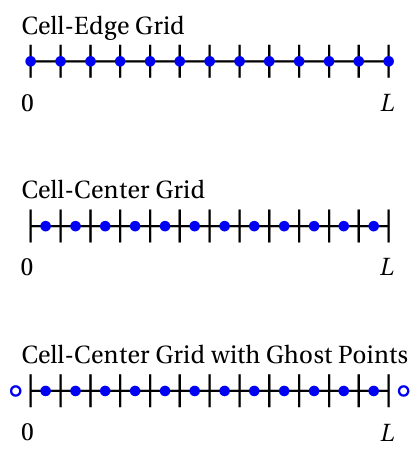
\includegraphics[width=\marginparwidth]{fig1}\captionof{figure}{Three commonspatial grids}\label{fig:1}}
    
    We\rq ll encounter three basic types of spatial grids in this class. Figure \ref{fig:1} shows a graphical representation of these three types of spatial grids for the region 
    \begin{math}0\leqslant x \leqslant l \end{math} . We divide this region into spatial cells (the spaces between vertical lines) and functions are evaluated at N discrete grid points (the dots). In a celledge grid, the grid points are located at the edge of the cell. In a cell-center grid, the points are located in the middle of the cell. Another useful grid is a cell-center grid with ghost points. The ghost points (unfilled dots) are extra grid points on either side of the interval of interest and are useful when we need to consider the derivatives at the edge of a grid.

      \begin{problem} \label{P1.2}
    \begin{enumerate}[label=(\alph*)]
    
      \item  Write a Python program that creates a cell-edge spatial grid in the variable x as follows: 
      \begin{lstlisting}
      	import numpy as np
      	
      	N=100
      	a=0
      	b=np.pi
      	x,h = np.linspace(a,b,N,retstep = True)
 		\end{lstlisting}
      Plot the function y(x) = sin(x)sinh(x) on this grid. Explain the relationship between the number of cells and the numberofgridpoints in a cell-edge grid.

    
    \marginpar{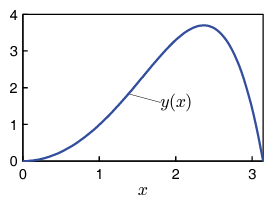
\includegraphics[width=\marginparwidth]{fig2}\captionof{figure}{Plot from 1.2(a)}\label{fig:2}} 
     
      \item     Explain the relationship between the number of cells and the number of grid points in a cell-center grid. Then write some code using NumPy\rq s arange function to create a cell-centered grid that has exactly 100 cells over the interval 0	$\geq$ x 	$\geq$ 2. 
           \\Evaluate the function f (x)=cosx on this grid and plot this function. Thenestimate the area under the curve by summingtheproductsof the centered function values fj with the widths of the cells h like this (midpoint integration rule):
      
      \begin{lstlisting}
      	np.sum(f)*h
      \end{lstlisting}
      
      Comparethis result to the exact answer obtained by integration: 
      \\      \[A = \int_0^2 cosx \ dx = sin(x) \vert_0^2 = sin(2) \]          
       
\item Build a cell-center grid with ghost points over the interval 0 $\geq$ x $\geq$ $\pi/2$ with 500 cells (502 grid points), and evaluate the function $f (x)=sinx$ on this grid. Now look carefully at the function values at the first two grid points and at the last two grid points. The function sinx has the property that $f(0) = 0$ and $f\prime(\pi/2) = 0$. The cell-center grid doesn\rq t have points at the ends of the interval, so these boundary conditions on the function need to be enforced using more than one point. Explain how the ghost points can be usedinconnectionwith interior points to specify both function-value boundary conditions andderivative-value boundary conditions.	    
    \end{enumerate}  
  \end{problem}
    \marginpar{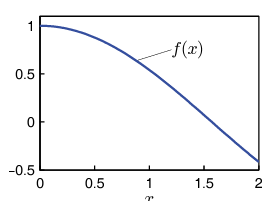
\includegraphics[width=\marginparwidth]{fig3}\captionof{figure}{Plot from 1.2(b)}\label{fig:3}}
    
 		\section*{Interpolation and extrapolation}
    \addcontentsline{toc}{section}{Interpolation and extrapolation}   
     
    Grids only represent functions at discrete points, and there will be times when we want to find good values of a function between grid points (interpolation) or beyond the last grid point (extrapolation). We will use interpolation and extrapolation techniques fairly often during this course, so let\rq s review these ideas. Thesimplest way to estimate function values is to use the fact that two points defineastraight line. For example, suppose that we have function values ($x_1$,$y_1$) and ($x_2$,$y_2$). The formula for a straight line that passes through these two points is   
    
\begin{equation} \label{eq:1}
    y - y_1 = \frac{(y_2-y_1)}{(x_2-x_1)}(x-x_1) 
\end{equation}  
  
    Once this line has been established it provides an approximation to the true function $y(x)$ that is pretty good in the neighborhood of the two data points. To linearly interpolate or extrapolate we simply evaluate Eq. \eqref{eq:1} at x values between or beyond $x_1$ and $x_2$.   
      
    \begin{problem} \label{P1.3} UseEq. \eqref{eq:1} to do the following special cases:
     
     \begin{enumerate}[label=(\alph*)]
     
     	\item Find an approximate value for $y(x)$ halfway between the two points $x_1$ and $x_2$. Does your answer make sense?
     	
     	\item Find an approximate value for $y(x)$ 3/4 of the way from $x_1$ to $x_2$. Do you see a pattern?
     	
     \marginpar{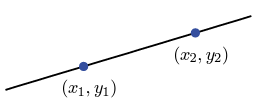
\includegraphics[width=\marginparwidth]{fig4}\captionof{figure}{The line defined bytwo points can be usedtointerpolate betweenthepoints andextrapolate beyond the points.}\label{fig:4}}
     
     	\item If the spacing between grid points is h (i.e. $x_2 − x_1 = h$), show that the linear extrapolation formula for $y(x2+h)$ is
     	
     	\begin{equation} \label{eq:2}
     		y(x_2 + h) = 2y_2 - y_1
     	\end{equation}
     	
     	This provides a convenient way to estimate the function value one grid step beyond the last grid point. Also show that
     	
     	\begin{equation} \label{eq:3}
     		y(x_2 + h/2) = 3y_2/2 - y_1/2
     	\end{equation}
     	
     	We will use both of these formulas during the course.
     	
     \end{enumerate}
    \end{problem}
     \section*{Derivatives on grids}
    \addcontentsline{toc}{section}{Derivatives on grids}  
     
	     Whensolving partial differential equations, we will frequently need to calculate derivatives on our grids. In your introductory calculus book, the derivative was probably introduced using the forward difference formula
		\begin{equation} \label{eq:4}
			f/prime(x) \approx \frac{f(x+h) - f(x)}{h}
		\end{equation}		     
     The word 	$''$ forward	$''$  refers to the way this formula reaches forward from $x$ to $x+h$ to calculate the slope. The exact derivative represented by Eq.\eqref{eq:4} in the limit that h approaches zero. However, wecan\rq t make h arbitrarily small when we represent a function on agrid because $(i)$ the number of cells needed to represent a region of space becomes infinite ash goes to zero; and $(ii)$ computers represent numbers with a finite number of significant digits so the subtraction in the numerator of Eq.\eqref{eq:4} loses accuracy when the two function values are very close. But given these limitation we want to be as accurate as possible, so we want to use the best derivative formulas available. The forward difference formula isn’t one of them.The best first derivative formula that uses only two function values is usually the centered difference formula:
     \begin{equation} \label{eq:5}
     	f\prime(x) \approx \frac{f(x+h)-f(x-h)}{2h} 
     \end{equation}
     It is called $''$centered$''$ because the point x at which we want the slope is centered between the places where the function is evaluated. Take a minute to study Fig. 1.5 to understand visually why the centered difference formula is so much better than the forward difference formula. The corresponding centered second derivative formula is
\marginpar{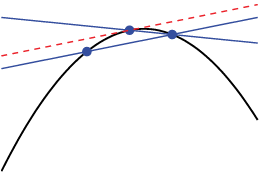
\includegraphics[width=\marginparwidth]{fig5}\captionof{figure}{The forward andcentered difference formulas both approximate the derivative as the slope of a line connecting two points. The centered difference formula gives a moreaccurate approximation because it uses points before and after the point where the derivative is being estimated. (The true derivative is the slope of the dotted tangent line).}\label{fig:5}}
\begin{equation} \label{eq:6}
	f\prime\prime(x) \approx \frac{f(x+h) - 2f(x)+f(x-h)}{h^2}
\end{equation}
We will derive both of these formulas later, but for now we just want you to understand how to use them. The colon operator provides a compact way to evaluate Eqs. \eqref{eq:5} and \eqref{eq:6} on a grid. Unfortunately for those of you familiar with Matlab, Python$'$ s colon operator acts a little differently from Matlab$'$ s in that the last index is not included in the range, as we noted in the tutorial. If the function we want to take the derivative of is stored in an array f, we can calculate the centered first derivative like this (remember that Python array indexes are zero-based):
\begin{lstlisting}
fp = np.zeros_like(f)
fp[1:N-1]=(f[2:N]-f[0:N-2])/(2*h)
\end{lstlisting}
and the centered second derivative at each interior grid point like this:
\begin{lstlisting}
fpp = np.zeros_like(f) 
fpp[1:N-1]=(f[2:N]-2*f[1:N-1]+f[0:N-2])/h**2
\end{lstlisting}

The variable h is the spacing between grid points and N is the number of grid points. Study this code (focus on the indexing) until you are convinced that it represents Eqs. \eqref{eq:5} and \eqref{eq:6} correctly. \\The derivative at the first and last points on the grid can\rq t be calculated with Eqs.  \eqref{eq:5} and \eqref{eq:6} since there are not grid points on both sides of the endpoints. Instead, we extrapolate the interior values of the two derivatives to the end points. If we use linear extrapolation then we just need two nearby points, and the formulas for the derivatives at the end points are found using Eq. \eqref{eq:2}
\begin{lstlisting}
fp[0]=2*fp[1]-fp[2] 
fp[N-1]=2*fp[N-2]-fp[N-3] 
fpp[0]=2*fpp[1]-fpp[2] 
fpp[N-1]=2*fpp[N-2]-fpp[N-3]
\end{lstlisting}

\begin{problem} \label{P1.4}
Create a cell-edge grid with N = 20 on the interval $0 \leq x \leq 5$. Load $f(x)$ with the Bessel function $J_0(x)$ and numerically differentiate it to obtain $f^\prime(x)$ and $f^\prime\prime(x)$. Then make overlaid plots of the numerical derivatives with the exact derivatives:
\end{problem}

\begin{equation*}
\begin{split}
			f^\prime(x) = -J_1(x)\\
			f^{\prime\prime} = \frac{1}{2}(-J_0(x)+J_2(x))	
			\end{split}
\end{equation*}
\marginpar{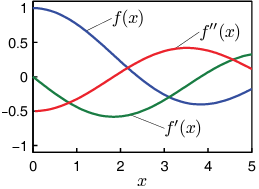
\includegraphics[width=\marginparwidth]{fig6}\captionof{figure}{Plots from 1.4}\label{fig:6}}

\section*{Errors in the approximate derivative formulas}
\addcontentsline{toc}{section}{Errors in the approximate derivative formulas}  

We\rq ll conclude this lab with a look at where the approximate derivative formulas come from and at the types of the errors that pop up when using them. The starting point is Taylor\rq expansion of the function f a small distance h away from the point x
\begin{equation}\label{eq:7}
	f(x+h) = f(x) + f^\prime(x)h+\frac{1}{2}f^{\prime\prime}(x)h^2 + ... + f^{(n)}(x)\frac{h^n}{n!} + ...
\end{equation}
Let\rq s use this series to understand the forward difference approximation to $f^\prime(x)$. If we apply the Taylor expansion to the $f(x+h)$ term in Eq. \eqref{eq:4} , we get
\begin{equation}\label{eq:8}
\frac{f(x+h) - f(x)}{h}= \frac{[f(x)+f^\prime(x)h+\frac{1}{2}f^{\prime\prime}(x)h^2+...]-f(x)}{h}
\end{equation}
The higher order terms in the expansion (represented by the dots) are smaller than the $f^{\prime\prime}$ term because they are all multiplied by higher powers of h (which we assumetobesmall). If we neglect these higher order terms, we can solve Eq. \eqref{eq:8} for the exact derivative $f^{\prime}(x)$ to find
\begin{equation}\label{eq:9}
f^\prime(x) \approx \frac{f(x+h)-f(x)}{h}-\frac{h}{2}f^{\prime\prime}(x)
\end{equation}
FromEq. \eqref{eq:9} we see that the forward difference does indeed give the first derivative back, but it carries an error term which is proportional to h. But if h is small enough then the contribution from the term containing $f^{\prime\prime}(x)$ will be too small to matter and we will have a good approximation to $f^\prime(x)$. For the centered difference formula, we use Taylor expansions for both $f(x+h)$ and $f(x−h)$in Eq. \eqref{eq:5} to write
\begin{equation} \label{eq:10}
	\frac{f(x+h)-f(x-h)}{2h} = \frac{[f(x)+f^\prime(x)h+f^{\prime\prime}(x)\frac{h^2}{2}+f^{\prime\prime\prime}(x)\frac{h3}{6}+...]}{2h}-\frac{[f(x)-f^\prime(x)h+f^{\prime\prime}(x)\frac{h^2}{2}-f^{\prime\prime\prime}(x)\frac{h3}{6}+...]}{2h}
\end{equation}
If we again neglect the higher-order terms, we can solve Eq. \eqref{eq:10} for the exact derivative $f^\prime(x)$. This time, we find that the $f^{\prime\prime}$ terms exactly cancel to give
\begin{equation} \label{eq:11}
	f^\prime \approx \frac{f(x+h) - f(x-h)}{2h} - \frac{h^2}{6} f^{\prime\prime\prime}(x) 
\end{equation}
Notice that for the centered formula the error term is much smaller, only of order $h^2$. So if we decrease h in both the forward and centered difference formulas by a factor of 10, the forward difference error will decrease by a factor of 10, but the centered difference error will decrease by a factor of 100. This is the reason we try to use centered formulas whenever possible in this course.


\begin{problem} \label{P1.5}
Write a Python program to compute the forward and centered difference formulas for the first derivative of the function $f(x) = e^x $ at $x = 0$ with $h = 0.1, 0.01, 0.001$. Verify that the error estimates in Eqs. \eqref{eq:9} and \eqref{eq:11} agree with the numerical testing. Note that at $x =0$ the exact values of both $f^\prime$ and $f^{\prime\prime}$ are equal to $e^0 = 1$,so just subtract 1 from your numerical result to find the error.

\end{problem}
\marginpar{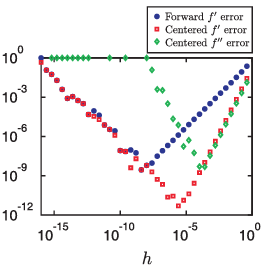
\includegraphics[width=\marginparwidth]{fig7}\captionof{figure}{Error in the forward and centered difference approximations to the first derivative and the centered difference formula for the second derivative as a function of h. Thefunction is $e^x$ and the approximations are evaluated for $x = 0$.}\label{fig:7}}

In problem 1.5, you found that $h = 0.001$ in the centered-difference formula gives a better approximation than $h=0.01$. This trend might entice you to try to keep making h smaller and smaller to achieve any accuracy you want. This doesn\rq t work. Figure \ref{fig:7} shows a plot of the error you calculated in problem 1.5 as h continues to decrease (note the log scales). For the larger values of h, the errors track well with the predictions made by the Taylor\rq s series analysis. However, when h becomes too small, the error starts to increase. By about $h=10−16$, and sooner for the second derivative, the error is the same order as the derivative. Thereason for this behavior is that numbers in computers are represented with a finite number of significant digits. Most computational languages (including Python) use double precision variables, which have 15-digit accuracy.\footnote{A computer uses 64 bits to represent a double precision number. 53 bits are used to represent the significant digits. Thus the significant digit part can be any integer between 0 and 253 = 9007199254740992 (almost 16 digits). The exponent is represented by 11 bits. After you add the possibility of NaN and Inf, the exponent can be −308 to +308. This leaves 1 bit for the overall sign of the number. Extended precision uses more bits (memory) and computation time, so double precision is mostly the standard for computational physics.} This is normally plenty of precision, but look what happens in a subtraction problem where the two numbers are nearly the same:
\begin{equation} \label{eq:12}
\opsub{7.38905699669556}{7.38905699191745}
\end{equation}
Notice that our nice 15-digit accuracy has disappeared, leaving behind only 6 significant figures. This problem occurs in calculations with floating-point numbers on all digital computers, and is called roundoff. You can see this effect by experimenting with the Python console:
\begin{lstlisting}
h=1e-17
g=1+h
print(g-1)
\end{lstlisting}
for different values of h and noting that you don\rq t always get h back. Also notice in Fig. 1.7 that this problem is worse for the second derivative formula than it is for the first derivative formula. The lesson here is that it is impossible to achieve arbitrarily high accuracy by using arbitrarily tiny values of h.
